\documentclass[10pt,aspectratio=169]{ntuabeamer}

\usepackage{booktabs}
\usepackage{tikz}
\usetikzlibrary{arrows.meta,positioning}

\graphicspath{{assets/}{assets/generated/}}

\definecolor{softblue}{HTML}{5B8DB8}
\definecolor{softteal}{HTML}{63A6A0}
\definecolor{softgold}{HTML}{D7A85E}
\definecolor{softcoral}{HTML}{C77C6B}
\definecolor{softpurple}{HTML}{8B82A8}
\definecolor{softink}{HTML}{263746}

\framesource{rumelhart1986}{Rumelhart, Hinton, Williams. \emph{Learning Representations by Back-Propagating Errors}. Nature, 1986.}
\framesource{kingma2015}{Kingma, Ba. \emph{Adam: A Method for Stochastic Optimization}. ICLR, 2015.}
\framesource{srivastava2014}{Srivastava et al. \emph{Dropout: A Simple Way to Prevent Neural Networks from Overfitting}. JMLR, 2014.}

\title{03 · Training Neural Networks}
\subtitle{Losses, backpropagation, optimization, and generalization}
\author{NTUA School of Civil Engineering}
\date{\today}

\begin{document}

\begin{frame}[plain]
  \makepresentationtitle
\end{frame}

\begin{frame}{Training Is a Feedback Loop}
  \begin{center}
  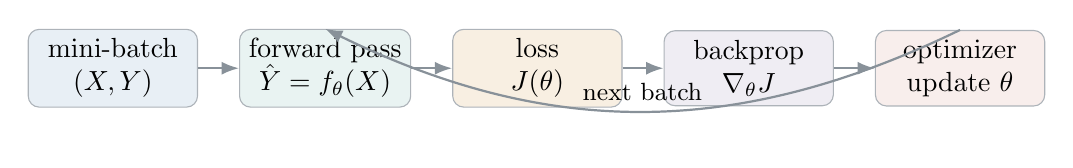
\begin{tikzpicture}[
    stage/.style={rounded corners, draw=softink!38, minimum width=2.15cm, minimum height=0.88cm, align=center},
    arrow/.style={-{Latex[length=2.2mm]}, thick, draw=softink!55}, node distance=0.52cm
  ]
    \node[stage, fill=softblue!14] (batch) {mini-batch\\$(X,Y)$};
    \node[stage, fill=softteal!14, right=of batch] (forward) {forward pass\\$\hat Y=f_\theta(X)$};
    \node[stage, fill=softgold!18, right=of forward] (loss) {loss\\$J(\theta)$};
    \node[stage, fill=softpurple!14, right=of loss] (back) {backprop\\$\nabla_\theta J$};
    \node[stage, fill=softcoral!13, right=of back] (update) {optimizer\\update $\theta$};
    \foreach \a/\b in {batch/forward,forward/loss,loss/back,back/update} \draw[arrow] (\a) -- (\b);
    \draw[arrow, bend left=26] (update.north) to node[above, font=\small] {next batch} (forward.north);
  \end{tikzpicture}
  \end{center}
  \begin{itemize}
    \item The forward pass computes predictions and records intermediate values.
    \item Backpropagation computes derivatives; it does not choose the update rule.
    \item The optimizer uses those derivatives to change the parameters.
  \end{itemize}
\end{frame}

\sectiondivider{Loss Functions}

\begin{frame}{Regression: Mean Squared Error}
  For $m$ output components:
  \[
    \ell_i=\frac12\lVert\hat{\mathbf y}_i-\mathbf y_i\rVert_2^2,
    \qquad
    J=\frac1n\sum_{i=1}^{n}\ell_i.
  \]
  \[
    \nabla_{\hat{\mathbf y}_i}\ell_i
    =\hat{\mathbf y}_i-\mathbf y_i.
  \]
  \begin{itemize}
    \item The square strongly penalizes large residuals.
    \item Targets with different physical units or scales require deliberate scaling or weighting.
    \item MSE is sensitive to outliers; absolute or robust losses may fit some noise models better.
  \end{itemize}
\end{frame}

\begin{frame}{Binary Classification: Logits and Cross-Entropy}
  With logit $z$, probability $p=\sigma(z)$, and label $y\in\{0,1\}$:
  \[
    \ell=-y\log p-(1-y)\log(1-p).
  \]
  The useful simplification is
  \[
    \frac{\partial\ell}{\partial z}=p-y.
  \]
  \begin{block}{Numerical stability}
    Use a library's ``binary cross-entropy with logits'' operation. It combines sigmoid and logarithms without rounding $p$ to exactly zero or one.
  \end{block}
\end{frame}

\begin{frame}{Multiclass Classification: Softmax Cross-Entropy}
  For logits $\mathbf z\in\mathbb R^C$:
  \[
    p_c=\frac{e^{z_c}}{\sum_{j=1}^{C}e^{z_j}},
    \qquad
    \ell=-\sum_{c=1}^{C}y_c\log p_c=-\log p_{y}.
  \]
  With a one-hot target vector $\mathbf y$:
  \[
    \nabla_{\mathbf z}\ell=\mathbf p-\mathbf y.
  \]
  Subtracting $\max_c z_c$ before exponentiation leaves $\mathbf p$ unchanged and prevents overflow.
\end{frame}

\begin{frame}{The Loss Must Match the Question}
  \centering
  \small
  \begin{tabular}{lll}
    \toprule
    Question & Output representation & Typical loss \\
    \midrule
    numerical prediction & real vector & MSE / robust regression loss \\
    one of two classes & one logit & binary cross-entropy \\
    exactly one of $C$ classes & $C$ logits & softmax cross-entropy \\
    several independent labels & $C$ logits & $C$ binary cross-entropies \\
    \bottomrule
  \end{tabular}
  \par
  \vspace{0.4cm}
  Multi-label classification is not multiclass classification: several labels may be true simultaneously, so a softmax is inappropriate.
\end{frame}

\sectiondivider{Backpropagation}

\begin{frame}{The Chain Rule on a Computation Graph}
  Let
  \[
    z=wx+b,\qquad a=\phi(z),\qquad \ell=\tfrac12(a-y)^2.
  \]
  Then
  \[
    \frac{\partial\ell}{\partial w}
    =\underbrace{(a-y)}_{\partial\ell/\partial a}
     \underbrace{\phi'(z)}_{\partial a/\partial z}
     \underbrace{x}_{\partial z/\partial w}.
  \]
  \begin{center}
  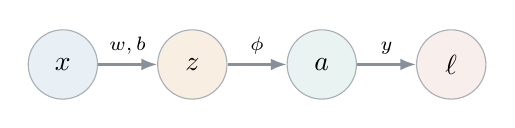
\begin{tikzpicture}[
    node distance=0.75cm,
    stage/.style={circle, draw=softink!40, minimum size=0.88cm},
    arrow/.style={-{Latex[length=2mm]}, thick, draw=softink!55}
  ]
    \node[stage, fill=softblue!14] (x) {$x$};
    \node[stage, fill=softgold!18, right=of x] (z) {$z$};
    \node[stage, fill=softteal!14, right=of z] (a) {$a$};
    \node[stage, fill=softcoral!13, right=of a] (l) {$\ell$};
    \draw[arrow] (x) -- node[above, font=\scriptsize] {$w,b$} (z);
    \draw[arrow] (z) -- node[above, font=\scriptsize] {$\phi$} (a);
    \draw[arrow] (a) -- node[above, font=\scriptsize] {$y$} (l);
  \end{tikzpicture}
  \end{center}
\end{frame}

\begin{frame}{Backpropagation Reuses Downstream Sensitivities\framecite{rumelhart1986}}
  For
  \[
    \mathbf z^{(\ell)}=W^{(\ell)}\mathbf a^{(\ell-1)}+\mathbf b^{(\ell)},
    \qquad
    \mathbf a^{(\ell)}=\phi^{(\ell)}(\mathbf z^{(\ell)}),
  \]
  define
  \[
    \boldsymbol\delta^{(\ell)}
    :=\nabla_{\mathbf z^{(\ell)}}\ell.
  \]
  Starting from the output sensitivity $\boldsymbol\delta^{(L)}$, move backward:
  \[
    \boldsymbol\delta^{(\ell)}=
    \left(W^{(\ell+1)}\right)^\top\boldsymbol\delta^{(\ell+1)}
    \odot \phi'^{(\ell)}(\mathbf z^{(\ell)}).
  \]
\end{frame}

\begin{frame}{Layer Gradients Have Simple Outer-Product Form}
  Once $\boldsymbol\delta^{(\ell)}$ is known:
  \[
    \nabla_{W^{(\ell)}}\ell
    =\boldsymbol\delta^{(\ell)}
      \left(\mathbf a^{(\ell-1)}\right)^\top,
    \qquad
    \nabla_{\mathbf b^{(\ell)}}\ell
    =\boldsymbol\delta^{(\ell)}.
  \]
  Shape check:
  \[
    \underbrace{d_\ell\times1}_{\boldsymbol\delta^{(\ell)}}
    \underbrace{1\times d_{\ell-1}}_{(\mathbf a^{(\ell-1)})^\top}
    =
    \underbrace{d_\ell\times d_{\ell-1}}_{\nabla_{W^{(\ell)}}\ell}.
  \]
  For a mini-batch, sum or average these per-example contributions according to the loss definition.
\end{frame}

\begin{frame}{Output Sensitivity Depends on Output and Loss}
  \centering
  \begin{tabular}{lll}
    \toprule
    Output & Loss & $\boldsymbol\delta^{(L)}$ \\
    \midrule
    linear & $\tfrac12\lVert\hat{\mathbf y}-\mathbf y\rVert^2$ & $\hat{\mathbf y}-\mathbf y$ \\
    sigmoid & binary cross-entropy & $p-y$ \\
    softmax & categorical cross-entropy & $\mathbf p-\mathbf y$ \\
    \bottomrule
  \end{tabular}
  \par
  \vspace{0.45cm}
  These compact expressions already include the derivative of the output activation.
\end{frame}

\begin{frame}{Automatic Differentiation Implements the Same Rule}
  \begin{enumerate}
    \item Forward operations create a computation graph and save required intermediate values.
    \item Reverse-mode automatic differentiation begins from the scalar loss.
    \item Each operation multiplies the incoming sensitivity by its local derivative.
    \item Contributions from several outgoing paths are added.
  \end{enumerate}
  \begin{block}{Why reverse mode?}
    Neural networks usually have one scalar loss and many parameters. One reverse traversal computes derivatives with respect to all parameters efficiently.
  \end{block}
  Gradient checking with finite differences is useful for new custom operations, but too expensive for routine training.
\end{frame}

\sectiondivider{Optimization}

\begin{frame}{Full-Batch, Stochastic, and Mini-Batch Gradients}
  For a batch $B$:
  \[
    \widehat{\nabla J}(\boldsymbol\theta)
    =\frac{1}{|B|}\sum_{i\in B}\nabla_{\boldsymbol\theta}\ell_i.
  \]
  \begin{itemize}
    \item full batch: $B$ is the entire training set
    \item stochastic: $|B|=1$
    \item mini-batch: intermediate size, efficient on vector hardware
  \end{itemize}
  An \textbf{iteration} performs one update; an \textbf{epoch} processes approximately one pass through the training set.
\end{frame}

\begin{frame}{Gradient Descent and Momentum}
  Plain gradient descent:
  \[
    \boldsymbol\theta_{t+1}
    =\boldsymbol\theta_t-\eta\mathbf g_t.
  \]
  Momentum:
  \[
    \mathbf v_{t+1}=\beta\mathbf v_t+\mathbf g_t,
    \qquad
    \boldsymbol\theta_{t+1}=\boldsymbol\theta_t-\eta\mathbf v_{t+1}.
  \]
  \begin{itemize}
    \item learning rate $\eta$ controls update scale
    \item momentum $\beta$ smooths directions across iterations
    \item gradients must be cleared before accumulating the next mini-batch in common autodiff libraries
  \end{itemize}
\end{frame}

\begin{frame}{Optimizer Geometry}
  \begin{figure}
    \centering
    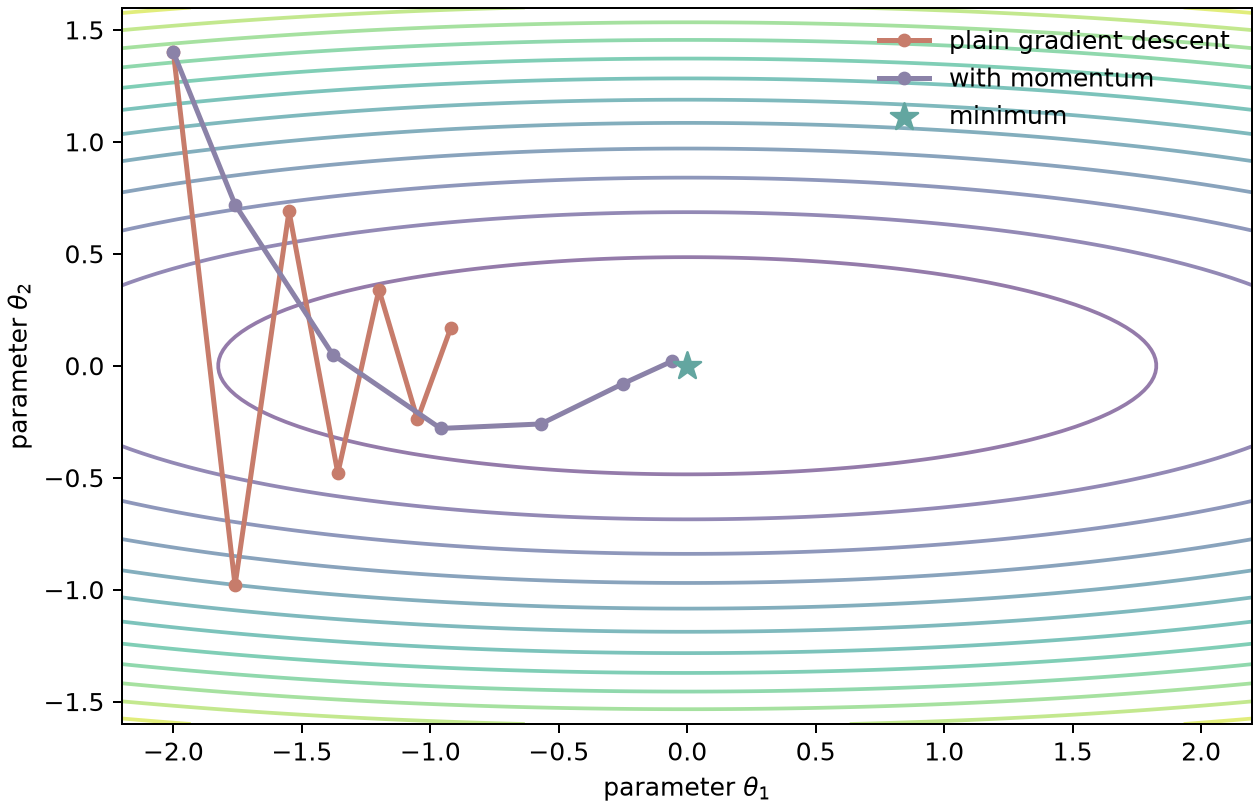
\includegraphics[width=0.59\linewidth]{optimizer_paths.png}
  \end{figure}
  \vspace{-0.35cm}
  Momentum can reduce oscillation across steep directions while preserving movement along a shallow valley.
\end{frame}

\begin{frame}{Adam: Adaptive Moments\framecite{kingma2015}}
  \small
  \[
    \mathbf m_t=\beta_1\mathbf m_{t-1}+(1-\beta_1)\mathbf g_t,
    \qquad
    \mathbf v_t=\beta_2\mathbf v_{t-1}+(1-\beta_2)\mathbf g_t^2,
  \]
  \[
    \hat{\mathbf m}_t=\frac{\mathbf m_t}{1-\beta_1^t},
    \qquad
    \hat{\mathbf v}_t=\frac{\mathbf v_t}{1-\beta_2^t},
  \]
  \[
    \boldsymbol\theta_{t+1}=\boldsymbol\theta_t-
    \eta\frac{\hat{\mathbf m}_t}{\sqrt{\hat{\mathbf v}_t}+\varepsilon}.
  \]
  Squares and divisions are element-wise. Adam is a useful default, not a guarantee of the best generalization.
\end{frame}

\begin{frame}{Learning Rate Is Usually the First Knob}
  \begin{columns}[T]
    \column{0.31\textwidth}
    \begin{block}{Too small}
      slow progress; training loss decreases steadily but barely
    \end{block}
    \column{0.31\textwidth}
    \begin{block}{Useful range}
      fast decrease followed by stable refinement
    \end{block}
    \column{0.31\textwidth}
    \begin{block}{Too large}
      oscillation, divergence, or non-finite loss
    \end{block}
  \end{columns}
  \vspace{0.35cm}
  Learning-rate schedules change $\eta$ during training; they do not replace validation-based model selection.
\end{frame}

\sectiondivider{Generalization and Regularization}

\begin{frame}{Capacity: Too Little, Useful, Too Much}
  \begin{figure}
    \centering
    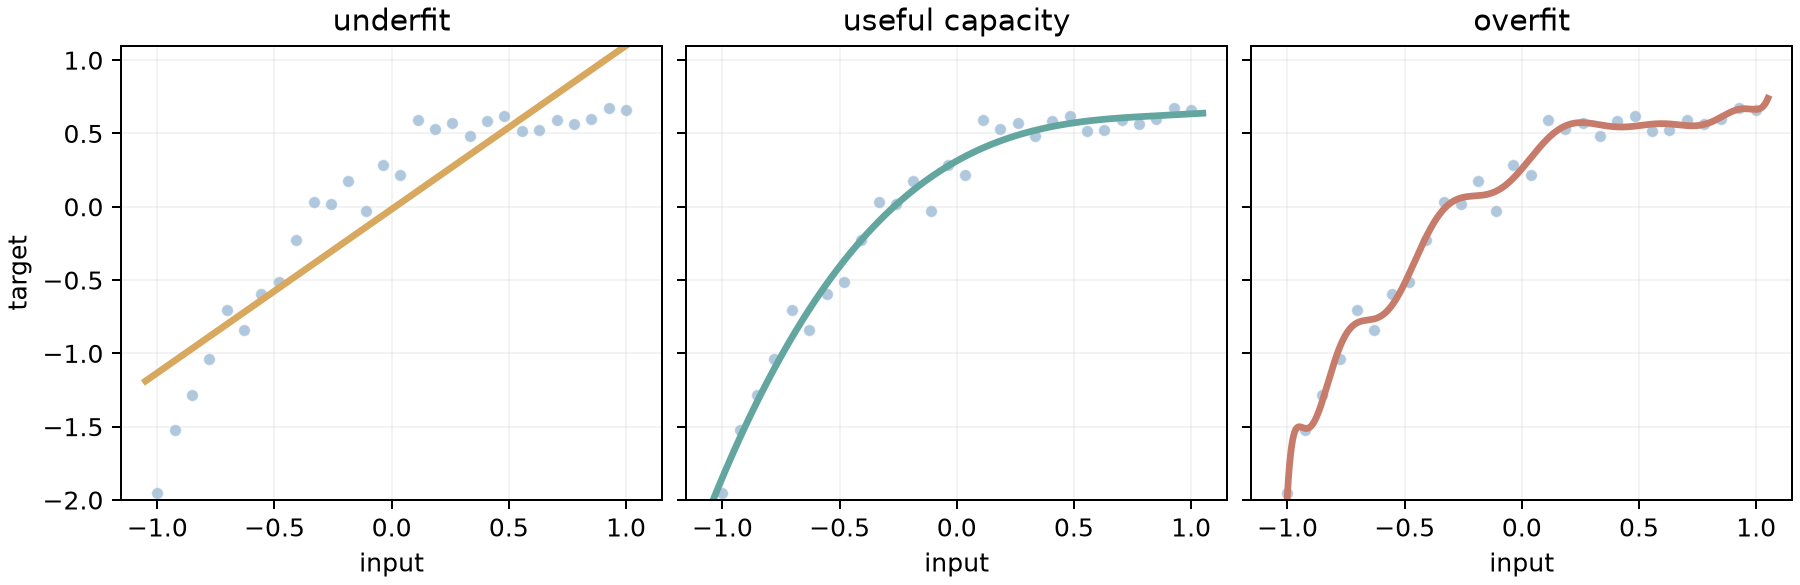
\includegraphics[width=0.9\linewidth]{capacity_tradeoff.png}
  \end{figure}
  \vspace{-0.3cm}
  \begin{itemize}
    \item Underfitting: training and validation errors are both high.
    \item Overfitting: training error is low while validation error deteriorates.
    \item Test data are not used to diagnose or repair either problem.
  \end{itemize}
\end{frame}

\begin{frame}{Data Protocol Prevents Optimistic Results}
  \begin{enumerate}
    \item Split independent units before fitting any preprocessing.
    \item Fit normalization, feature selection, and augmentation policy on training data.
    \item Select architecture and hyperparameters using validation performance.
    \item Freeze the full pipeline.
    \item Evaluate once on the test set and report uncertainty where practical.
  \end{enumerate}
  \begin{alertblock}{Common leakage}
    Computing normalization statistics on all data, splitting overlapping time windows independently, or choosing checkpoints using test performance.
  \end{alertblock}
\end{frame}

\begin{frame}{$L_2$ Penalty and Weight Decay}
  A penalized objective can be written
  \[
    \widetilde J(\boldsymbol\theta)
    =J(\boldsymbol\theta)+\frac{\lambda}{2}\lVert\mathbf w\rVert_2^2,
  \]
  giving
  \[
    \nabla_{\mathbf w}\widetilde J
    =\nabla_{\mathbf w}J+\lambda\mathbf w.
  \]
  \begin{itemize}
    \item discourages large weights rather than forbidding them
    \item biases are usually excluded
    \item coupled $L_2$ regularization and decoupled weight decay are equivalent for plain SGD, but not generally for adaptive optimizers
  \end{itemize}
\end{frame}

\begin{frame}{Dropout Trains Random Subnetworks\framecite{srivastava2014}}
  During training, for keep probability $q$:
  \[
    \mathbf m\sim\operatorname{Bernoulli}(q),
    \qquad
    \tilde{\mathbf h}=\frac{\mathbf m\odot\mathbf h}{q}.
  \]
  \begin{itemize}
    \item inverted scaling keeps $\mathbb E[\tilde{\mathbf h}]=\mathbf h$
    \item dropout is disabled for ordinary deterministic evaluation
    \item it is one regularizer, not a required ingredient in every architecture
  \end{itemize}
\end{frame}

\begin{frame}{Data Augmentation Must Preserve the Label}
  \begin{itemize}
    \item Images: small translations, crops, flips, or photometric changes when the task is invariant to them.
    \item Signals: physically defensible noise, scaling, or time shifts.
    \item Simulations: sample admissible parameters or boundary conditions.
  \end{itemize}
  \begin{alertblock}{Do not assume invariance}
    A horizontal flip changes left/right labels; an arbitrary time warp can change frequency content; noise beyond the sensor model can create impossible samples.
  \end{alertblock}
\end{frame}

\begin{frame}{Early Stopping Uses Validation Data}
  \begin{columns}
    \column{0.6\textwidth}
    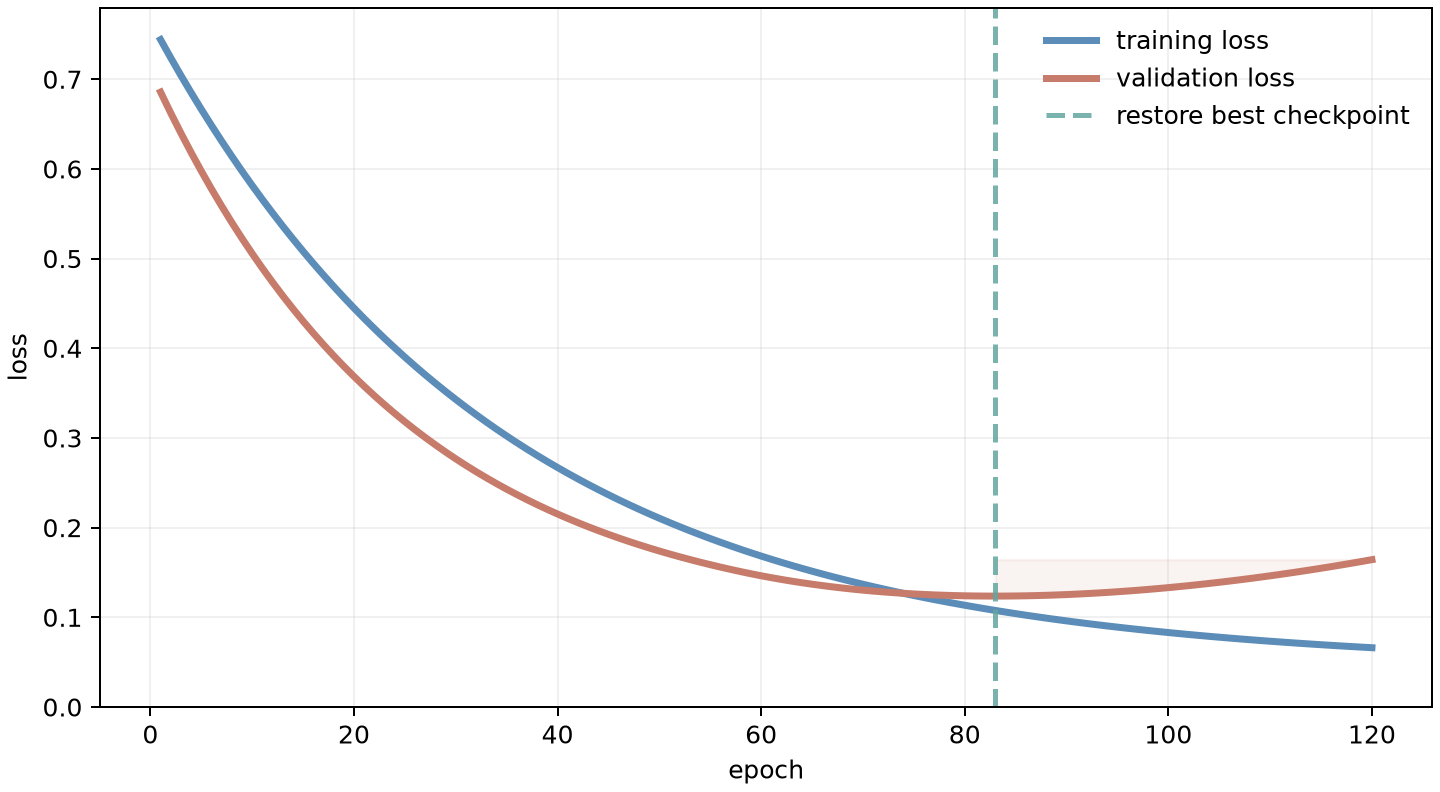
\includegraphics[width=\linewidth]{learning_curves.png}
    \column{0.37\textwidth}
    \begin{enumerate}
      \item monitor validation loss
      \item save the best checkpoint
      \item stop after no improvement for a chosen patience
      \item restore the best checkpoint, not the last one
    \end{enumerate}
  \end{columns}
\end{frame}

\begin{frame}{A Minimal Reliable Training Recipe}
  \begin{enumerate}
    \item Establish a simple baseline and a leakage-safe split.
    \item Normalize using training statistics.
    \item Verify tensor shapes and overfit one tiny batch as a debugging check.
    \item Choose a task-compatible output and loss.
    \item Train with mini-batches; monitor training and validation curves.
    \item Tune learning rate before adding complexity.
    \item Add only justified regularization.
    \item Restore the selected checkpoint and evaluate the test set once.
  \end{enumerate}
\end{frame}

\begin{frame}{Takeaways}
  \begin{itemize}
    \item The loss defines the prediction error; its scale and output parameterization matter.
    \item Backpropagation is reverse-mode chain rule with reused sensitivities.
    \item The optimizer consumes gradients; it is separate from backpropagation.
    \item Validation data guide choices. Test data estimate final generalization.
    \item Regularization trades training fit for more reliable unseen-data performance.
    \item Curves and simple debugging checks are more informative than adding architecture blindly.
  \end{itemize}
\end{frame}

\end{document}
